\section{Mobile Application \textit{Connected.Football}}
\label{sec:Product}
\lhead{Mobile Application \textit{Connected.Football}}
This chapter explains the \textit{Connected.Football} application in detail. The \textit{Connected.Football} application is used by football coaches for planning and communication with the team. 

\subsection{Architecture}
The \textit{Connected.Football} application was created with \textit{React Native}. \textit{React Native} is based on the \textit{JavaScript} library \textit{React} which is maintained by Facebook. \textit{React} can be used as a base for single-page websites and for mobile applications. 

\begin{figure}[H]
    \centering
    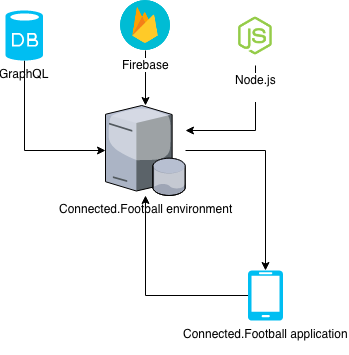
\includegraphics[width=0.55\textwidth,keepaspectratio]{content/pictures/architecture.png}
	\caption{\textit{Connected.Football} Architecture}
	\label{fig:connected_football_architecture}
\end{figure}

\textit{Connected.Football} also uses \textit{MongoDB} as a database for storing the members, the training programs and other data. \textit{GraphQL} is used to communicate between the \textit{Connected.Football} application and the database. 

\subsubsection{\textit{React Native}}
\label{sssec:react_native}

\textit{React Native} was announced by Facebook in 2015 and is using the \textit{React} architecture to crate native \textit{Android} and \textit{iOS} applications. 
\newline
The working principles of \textit{React Native} are basically the same as \textit{React} except that \textit{React Native} uses native views. It runs in a background process (which interprets the \textit{JavaScript} written by the developers) directly on the end-device.

\subsubsection{\textit{GraphQL}}
\label{sssec:graphql}

\textit{GraphQL} is a query language for APIs and a run time for fulfilling those queries with existing data. \textit{GraphQL} provides a complete and understandable description of the data in your API, gives clients the power to ask for exactly what they need and nothing more, makes it easier to evolve APIs over time, and enables powerful developer tools.